\documentclass{article}%
\usepackage[T1]{fontenc}%
\usepackage[utf8]{inputenc}%
\usepackage{lmodern}%
\usepackage{textcomp}%
\usepackage{lastpage}%
\usepackage[head=40pt,margin=0.5in,bottom=0.6in]{geometry}%
\usepackage{graphicx}%
%
\title{\textbf{Vecinos de Chacao salieron a protestar por falta de agua}}%
\author{El Nacional Web}%
\date{21/09/2018}%
%
\begin{document}%
\normalsize%
\maketitle%
\textbf{URL: }%
http://www.el{-}nacional.com/noticias/sociedad/vecinos{-}chacao{-}salieron{-}protestar{-}por{-}falta{-}agua\_252692\newline%
%
\textbf{Periodico: }%
EN, %
ID: %
252692, %
Seccion: %
Sociedad\newline%
%
\textbf{Palabras Claves: }%
Hidrocapital, Sociedad\newline%
%
\textbf{Derecho: }%
2.8, %
Otros Derechos: %
, %
Sub Derechos: %
2.8.1\newline%
%
\textbf{EP: }%
SI\newline%
\newline%
%
\textbf{\textit{El dirigente vecinal de la entidad indicó que no son escuchados por las autoridades competentes}}%
\newline%
\newline%
%
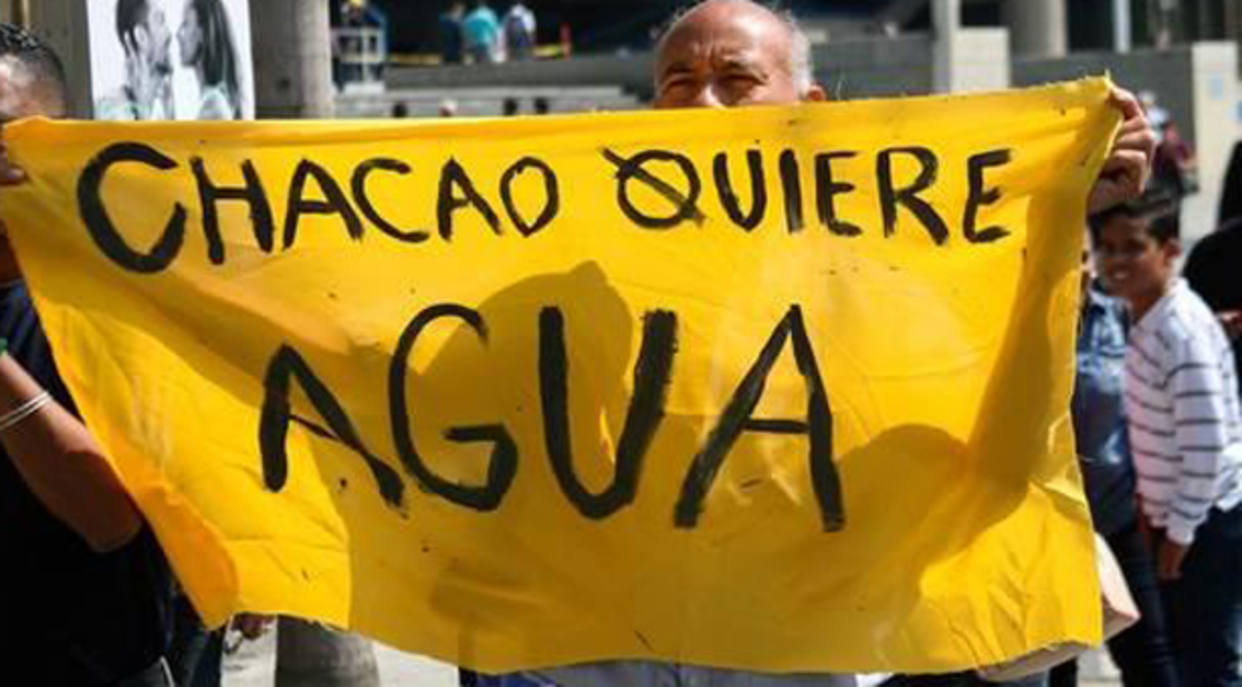
\includegraphics[width=300px]{32.jpg}%
\newline%
%
Habitantes del municipio Chacao, estado Miranda, protestaron este viernes~en la avenida Francisco de Miranda~para exigir el servicio de agua en la localidad.%
\newline%
%
Los ciudadanos aseguraron~que no tienen~agua desde hace varios meses por lo que~denunciaron que no son escuchados por la empresa estatal Hidrocapital.%
\newline%
%
Gabriel Santana, dirigente vecinal de la zona, comunicó que en los próximos días se llevará una carta al organismo para realizar la respectiva denunciar por la falta del servicio.%
\newline%
%
"Hay zonas que~desde hace dos y tres semanas no ven ni una sola gota, lo que representa que los colegios del municipio han tenido que cancelar clases por no tener agua", enfatizó Santana para~VPItv.%
\newline%
%
\end{document}